%!Mode:: "TeX:UTF-8"
% !TEX program  = xelatex
\documentclass[a4paper,11pt,UTF8,AutoFakeBold]{ctexart}

% 引入宏定义 macros.tex
% !TeX program = xelatex

\usepackage{indentfirst} %缩进
\usepackage{xeCJK}    %使用系统字体
\usepackage{bm}       %粗体
\usepackage{fancyhdr} %自定义页眉页脚
%\pagestyle{empty}    % 没有页眉页脚
\pagestyle{plain}     % 没有页眉,页脚包含一个居中的页码
\usepackage{amsmath, amsthm, amssymb, amsfonts} %数学公式
\usepackage[a4paper,left=3cm,right=3cm,top=3.5cm,bottom=3.5cm]{geometry}
\usepackage{booktabs} %插入表格
\usepackage[section]{placeins} %避免浮动
\usepackage{listings} %插入代码
\usepackage{underscore} % 在非数学环境下不再需要转义 '_'
\usepackage{ctex}     %中文宏包
\usepackage[svgnames, table]{xcolor} %彩色表格
\usepackage{algorithm}          %伪代码
\usepackage{algorithmicx}
\usepackage{algpseudocode}
\usepackage{algorithm,algpseudocode,float}
\usepackage{lipsum}
\usepackage{enumitem}           %调整列举环境
\usepackage{url}
\usepackage{fontspec,xunicode}
\usepackage{tabularx}            % 增强表格
\usepackage{multirow}            % 多行、多列
\defaultfontfeatures{Mapping=tex-text} %如果没有它,会有一些 tex 特殊字符无法正常使用,比如连字符。
\usepackage[explicit]{titlesec}
\usepackage[breaklinks,colorlinks,linkcolor=black,citecolor=black,urlcolor=black]{hyperref} % 生成 PDF 书签
\usepackage{float}
\usepackage{xifthen} % provides \isempty test



\usepackage{graphicx}
\graphicspath{{imgs/}}

%%%%%%%%%%%%%%%%%%%%%%%%%%%%%%%%%%%%%%%%%%%%%%%%%%%%%%%%%%%%%%%%
% 缩进及行间距
%%%%%%%%%%%%%%%%%%%%%%%%%%%%%%%%%%%%%%%%%%%%%%%%%%%%%%%%%%%%%%%%
\setlength{\parindent}{22bp} %重新定义缩进长度
\linespread{1}

%%%%%%%%%%%%%%%%%%%%%%%%%%%%%%%%%%%%%%%%%%%%%%%%%%%%%%%%%%%%%%%%
% 图的标题行间距设置
%%%%%%%%%%%%%%%%%%%%%%%%%%%%%%%%%%%%%%%%%%%%%%%%%%%%%%%%%%%%%%%%
\newcommand{\bottomcaption}{%
    \setlength{\abovecaptionskip}{6bp}%
    \setlength{\belowcaptionskip}{6bp}%
    \caption
}

%%%%%%%%%%%%%%%%%%%%%%%%%%%%%%%%%%%%%%%%%%%%%%%%%%%%%%%%%%%%%%%%
% 字体定义
%%%%%%%%%%%%%%%%%%%%%%%%%%%%%%%%%%%%%%%%%%%%%%%%%%%%%%%%%%%%%%%%
\setmainfont{Times New Roman}  %默认英文字体.serif是有衬线字体sans serif无衬线字体
\setmonofont{Consolas}
\setCJKmainfont[ItalicFont={宋体}, BoldFont={黑体}]{宋体}%衬线字体 缺省中文字体为 
% \punctstyle{hangmobanjiao}
%-----------------------xeCJK下设置中文字体------------------------------%
\setCJKfamilyfont{song}{SimSun}                             %宋体 song
\newcommand{\song}{\CJKfamily{song}}
\setCJKfamilyfont{fs}{FangSong}                      %仿宋  fs
\newcommand{\fs}{\CJKfamily{fs}}
\let\kaishu\relax                                    %重定义楷体,打开假粗体
\newCJKfontfamily\kaishu{KaiTi}[AutoFakeBold]
%\setCJKfamilyfont{ktgb}{KaiTi_GB2312}                      %楷体 GB2312
%\newcommand{\ktgb}{\CJKfamily{ktgb}}
\setCJKfamilyfont{yh}{Microsoft YaHei}                    %微软雅黑 yh
\newcommand{\yh}{\CJKfamily{yh}}
\setCJKfamilyfont{hei}{SimHei}                              %黑体  hei
\newcommand{\hei}{\CJKfamily{hei}}
\setCJKfamilyfont{hwxk}{STXingkai}                                %华文行楷  hwxk
\newcommand{\hwxk}{\CJKfamily{hwxk}}
\setCJKfamilyfont{fzshu}{FZShuTi}                                    %方正舒体 fzshu
\newcommand{\fzshu}{\CJKfamily{fzshu}}
%------------------------------设置字体大小------------------------%
\newcommand{\chuhao}{\fontsize{42bp}{63bp}\selectfont}     %初号, 1.5倍行距
\newcommand{\xiaochuhao}{\fontsize{36bp}{36bp}\selectfont} %小初号,单倍行距
\newcommand{\yihao}{\fontsize{26bp}{39bp}\selectfont}        % 一号, 1.5 倍行距
\newcommand{\erhao}{\fontsize{22bp}{33bp}\selectfont}        % 二号, 1.5倍行距
\newcommand{\xiaoerhao}{\fontsize{18bp}{18bp}\selectfont}       % 小二, 单倍行距
\newcommand{\sanhao}{\fontsize{16bp}{24bp}\selectfont}       % 三号, 1.5倍行距
\newcommand{\xiaosanhao}{\fontsize{15bp}{22bp}\selectfont}      % 小三, 1.5倍行距
\newcommand{\sihao}{\fontsize{14bp}{21bp}\selectfont}        % 四号, 1.5 倍行距
\newcommand{\banxiaosi}{\fontsize{13bp}{20bp}\selectfont}  % 半小四, 20pt行距
\newcommand{\xiaosihao}{\fontsize{12bp}{20bp}\selectfont}       % 小四, 20pt行距
\newcommand{\dawuhao}{\fontsize{11bp}{11bp}\selectfont}      % 大五号, 单倍行距
\newcommand{\wuhao}{\fontsize{10.5bp}{10.5bp}\selectfont}   % 五号, 单倍行距
\newcommand{\xiaowuhao}{\fontsize{9bp}{9bp}\selectfont}   %小五号,单倍行距
%------------------------------重定义normalize------------------------%
\renewcommand{\normalsize}{\fontsize{12bp}{20bp}\selectfont}


%%%%%%%%%%%%%%%%%%%%%%%%%%%%%%%%%%%%%%%%%%%%%%%%%%%%%%%%%%%%%%%%
% 图题字体大小相同
%%%%%%%%%%%%%%%%%%%%%%%%%%%%%%%%%%%%%%%%%%%%%%%%%%%%%%%%%%%%%%%%
\usepackage{caption}
\captionsetup{font={footnotesize}}   % footnotesize = 9bp
\captionsetup[lstlisting]{font={footnotesize}}

%%%%%%%%%%%%%%%%%%%%%%%%%%%%%%%%%%%%%%%%%%%%%%%%%%%%%%%%%%%%%%%%
% 重定义枚举编号为 1),2)...
%%%%%%%%%%%%%%%%%%%%%%%%%%%%%%%%%%%%%%%%%%%%%%%%%%%%%%%%%%%%%%%%
\renewcommand{\labelenumi}{\theenumi)}


%%%%%%%%%%%%%%%%%%%%%%%%%%%%%%%%%%%%%%%%%%%%%%%%%%%%%%%%%%%%%%%%
% 重定义section标题
%%%%%%%%%%%%%%%%%%%%%%%%%%%%%%%%%%%%%%%%%%%%%%%%%%%%%%%%%%%%%%%%
\CTEXsetup[format={\song\bfseries\zihao{4}},number={\chinese{section}},name={,、~},aftername={},indent={0bp},beforeskip={6bp},afterskip={6bp},format+={\flushleft}]{section}
\CTEXsetup[format={\Large\bfseries\song\zihao{5}},name={(,)},number={\chinese{subsection}},aftername={},indent={22bp},beforeskip={6bp},afterskip={6bp}]{subsection}
\CTEXsetup[format={\Large\bfseries\song\zihao{5}},name={,.},aftername={ },indent={28bp},beforeskip={6bp},afterskip={6bp}]{subsubsection}
\CTEXsetup[number={\chinese{section}},name={附录, ~~ }]{appendix}



%%%%%%%%%%%%%%%%%%%%%%%%%%%%%%%%%%%%%%%%%%%%%%%%%%%%%%%%%%%%%%%%
% 标题名称中文化
%%%%%%%%%%%%%%%%%%%%%%%%%%%%%%%%%%%%%%%%%%%%%%%%%%%%%%%%%%%%%%%%
\renewcommand\figurename{\hei 图}
\renewcommand\tablename{\hei 表}
\renewcommand\lstlistingname{\hei 代码}
\renewcommand{\algorithmicrequire}{\textbf{输入:}}
\renewcommand{\algorithmicensure}{\textbf{输出:}}
\newtheorem{define}{定义}


%%%%%%%%%%%%%%%%%%%%%%%%%%%%%%%%%%%%%%%%%%%%%%%%%%%%%%%%%%%%%%%%
% 列表设置
%%%%%%%%%%%%%%%%%%%%%%%%%%%%%%%%%%%%%%%%%%%%%%%%%%%%%%%%%%%%%%%%
\setlist[enumerate,1]{leftmargin=46bp,listparindent=0bp,itemsep=0mm,partopsep=.7mm,parsep=0ex,labelsep=1.5mm,topsep=0.7mm}
\setlist[enumerate,2]{label=\alph*),leftmargin=1.5em}  %二级item设置
\setitemize{leftmargin=46bp,listparindent=0bp,itemsep=0mm,partopsep=.7mm,parsep=0ex,labelsep=1.5mm,topsep=0.7mm}
\setitemize{itemindent=38bp,leftmargin=0bp,itemsep=-0.4ex,listparindent=26bp,partopsep=0bp,parsep=0.5ex,topsep=-0.25ex}
%\setdescription{itemindent=38bp,leftmargin=0bp,itemsep=-0.4ex,listparindent=26bp,partopsep=0bp,parsep=0.5ex,topsep=-0.25ex}

%%%%%%%%%%%%%%%%%%%%%%%%%%%%%%%%%%%%%%%%%%%%%%%%%%%%%%%%%%%%%%%%
% 代码设置
%%%%%%%%%%%%%%%%%%%%%%%%%%%%%%%%%%%%%%%%%%%%%%%%%%%%%%%%%%%%%%%%
\lstset{
 columns=fixed,
 numbers=left,                                        % 在左侧显示行号
 numberstyle=\tiny\color{gray},                       % 设定行号格式
 frame=single,                                        % 单线背景边框
 breaklines=true,                                     % 设定LaTeX对过长的代码行进行自动换行
 keywordstyle=\color[RGB]{40,40,255},                 % 设定关键字颜色
 numberstyle=\footnotesize\color{darkgray},
 commentstyle=\it\color[RGB]{0,96,96},                % 设置代码注释的格式
 stringstyle=\rmfamily\slshape\color[RGB]{128,0,0},   % 设置字符串格式
 showstringspaces=false,                              % 不显示字符串中的空格
 language=java,                                        % 设置语言
 basicstyle=\linespread{1.0}\xiaowuhao\ttfamily,                      % 字体字号
 %lineskip=10bp,
 %baselinestretch=1,
}


%%%%%%%%%%%%%%%%%%%%%%%%%%%%%%%%%%%%%%%%%%%%%%%%%%%%%%%%%%%%%%%%
% 伪代码分页
%%%%%%%%%%%%%%%%%%%%%%%%%%%%%%%%%%%%%%%%%%%%%%%%%%%%%%%%%%%%%%%%
\makeatletter
\renewcommand{\ALG@name}{算法}
\newenvironment{breakablealgorithm}
  {% \begin{breakablealgorithm}
   \begin{center}
     \refstepcounter{algorithm}% New algorithm
     \hrule height.8bp depth0bp \kern2bp% \@fs@pre for \@fs@ruled
     \renewcommand{\caption}[2][\relax]{% Make a new \caption
       {\raggedright\textbf{\ALG@name~\thealgorithm} ##2\par}%
       \ifx\relax##1\relax % #1 is \relax
         \addcontentsline{loa}{algorithm}{\protect\numberline{\thealgorithm}##2}%
       \else % #1 is not \relax
         \addcontentsline{loa}{algorithm}{\protect\numberline{\thealgorithm}##1}%
       \fi
       \kern2bp\hrule\kern2bp
     }
  }{% \end{breakablealgorithm}
     \kern2bp\hrule\relax% \@fs@post for \@fs@ruled
   \end{center}
  }
\makeatother


%%%%%%%%%%%%%%%%%%%%%%%%%%%%%%%%%%%%%%%%%%%%%%%%%%%%%%%%%%%%%%%%
% 设置 \part
%%%%%%%%%%%%%%%%%%%%%%%%%%%%%%%%%%%%%%%%%%%%%%%%%%%%%%%%%%%%%%%%

\titleformat{\part}[display]{}{}{0pt}{}
%\titlespacing*{\part}{0pt}{0pt}{0pt}   % 在正文中隐藏 part
\makeatletter
\@addtoreset{section}{part} % 使 section 在 part 后重新标号
\makeatother


%%%%%%%%%%%%%%%%%%%%%%%%%%%%%%%%%%%%%%%%%%%%%%%%%%%%%%%%%%%%%%%%
% 设置个人信息
%%%%%%%%%%%%%%%%%%%%%%%%%%%%%%%%%%%%%%%%%%%%%%%%%%%%%%%%%%%%%%%%
\makeatletter
\newcommand{\course}[1]{
    \newcommand{\report@course}{#1}
}
\newcommand{\college}[1]{
    \newcommand{\report@college}{#1}
}
\newcommand{\major}[1]{
    \newcommand{\report@major}{#1}
}
\newcommand{\studentid}[1]{
    \newcommand{\report@studentid}{#1}
}
%\newcommand{\theauthor}[1]{
%    \newcommand{\report@author}{#1}
%}
\newcommand{\teacher}[1]{
    \newcommand{\report@teacher}{#1}
}
\newcommand{\thedate}[1]{
    \newcommand{\report@date}{#1}
}
\makeatother


%%%%%%%%%%%%%%%%%%%%%%%%%%%%%%%%%%%%%%%%%%%%%%%%%%%%%%%%%%%%%%%%
% 设置 \maketitle
%%%%%%%%%%%%%%%%%%%%%%%%%%%%%%%%%%%%%%%%%%%%%%%%%%%%%%%%%%%%%%%%
\makeatletter
\renewcommand{\maketitle}{
    \thispagestyle{empty}   % 去掉首页页码
    \begin{titlepage}

        \begin{figure}[!htbp]
            \centering
            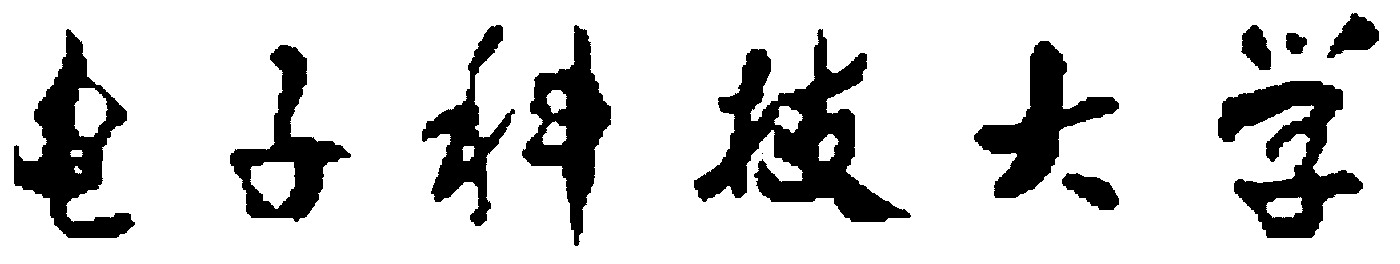
\includegraphics[width=\textwidth]{uestc}
        \end{figure}

        \center{\xiaochuhao{\kaishu 计算机专业类课程}}
        \vspace{1.5cm}
        \center{\fontsize{48bp}{52bp}{\song{\bfseries 实\\验\\报\\告}}}

        \vspace{1.5cm}

        \begin{center}
            \begin{large}
                \begin{tabular}{rl}
                    \xiaoerhao{\bfseries\fs{课程名称:}}& \xiaoerhao{\bfseries\hei{\report@course}}\\
                    \\
                    \xiaoerhao{\bfseries\fs{学\qquad 院:}}& \xiaoerhao{\bfseries\hei{\report@college}}\\
                    \\
                    \xiaoerhao{\bfseries\fs{学院专业:}}& \xiaoerhao{\bfseries\hei{\report@major}}\\
                    \\
                    \xiaoerhao{\bfseries\fs{学\qquad 号:}}& \xiaoerhao{\bfseries\hei{\report@studentid}}\\
                    \\
                    \xiaoerhao{\bfseries\fs{学生姓名:}}& \xiaoerhao{\bfseries\hei{\@author}}\\
                    \\
                    \xiaoerhao{\bfseries\fs{指导教师:}}& \xiaoerhao{\bfseries\hei{\report@teacher}}\\
                    \\
                    \xiaoerhao{\bfseries\fs{日\qquad 期:}}& \xiaoerhao{\bfseries\hei{\report@date}}\\
                \end{tabular}
            \end{large}
        \end{center}
    \end{titlepage}
    \newpage
    \setcounter{page}{1} % 第二页从 1 开始标号
}
\makeatother

%%%%%%%%%%%%%%%%%%%%%%%%%%%%%%%%%%%%%%%%%%%%%%%%%%%%%%%%%%%%%%%%
% 设置 \chapter
%%%%%%%%%%%%%%%%%%%%%%%%%%%%%%%%%%%%%%%%%%%%%%%%%%%%%%%%%%%%%%%%

\makeatletter
\newcommand{\chapter}[3]{
    \newpage
    \part{}
    \vspace*{-120bp} % Adjust the vertical space here
    \centerline{\\[40bp]\erhao{\fzshu{\bfseries 电 ~子 ~科~ 技~ 大~ 学}}}
    \vspace*{-20bp} % Adjust the vertical space her
    \centerline{\\[20bp]\yihao{\hei{\bfseries 实  ~~~ 验  ~~~ 报  ~~~ 告}}}

    % \ifthenelse{\isempty{#3}}{
    %     \centerline{\\[20bp]\yihao{\song{\bfseries #1}}}
    % }{
        \noindent
        \begin{tabularx}{\textwidth}{XXX}
            \Large\bfseries\song\zihao{4}学生姓名:{\@author} &
            \Large\bfseries\song\zihao{4}学 号:{\report@studentid} &
            \Large\bfseries\song\zihao{4}指导教师:{\report@teacher}
        \end{tabularx}\\

    %     \noindent
    %     \begin{tabularx}{\textwidth}{XX}
    %         \Large\bfseries\song\zihao{4}实验地点:{#2} &
    %         \Large\bfseries\song\zihao{4}实验时间:{#3}
    %     \end{tabularx}
    % }
}
\makeatother



\begin{document}
\xiaosihao \setCJKfamilyfont{song}{SimSun}  

\course{计算机视觉与模式识别}
\college{计算机科学与工程学院}
\major{计算机科学与技术}
\studentid{2022010910017}
\author{谢卿云}
\teacher{沈复民}
\thedate{2025 年 5 月 26 日}

% \maketitle

%\chapter{实验一}{}{}  % 用于单次实验报告开头的 “实验X”
\chapter{}{}{}           % 实验信息

\section{实验项目名称:}
Scene Recognition with Bag of Words

\section{实验原理:}
\subsection{Harris角点检测算法}
\subsubsection{概念}
在图像中,角点是指一个局部区域在两个或多个主要方向上都有显著的灰度变化的点。
简单来说,角点可以看作是两条边的交汇处。与平坦区域(在任何方向移动窗口,灰度变化都很小)
和边缘区域(只在一个方向上移动窗口有显著灰度变化)不同,
角点区域在任何方向上移动小窗口都会引起显著的灰度变化。
这使得角点成为图像中重要的、对平移、旋转和光照变化具有一定鲁棒性的特征点。
在本实验中,我们采用Harris角点作为兴趣点,完成对student.py/
\subsubsection{数学原理}
Harris角点检测的核心思想是,在一个像素点周围定义一个小的“窗口”。
然后,计算当这个窗口在水平和垂直方向上分别移动一个小的距离 \((u, v)\) 时,
窗口内的像素灰度值变化的平方和。
灰度变化函数 \(E(u,v)\) 可以表示为:

\[ E(u,v) = \sum_{x,y} w(x,y) [I(x+u, y+v) - I(x,y)]^2 \]
    
其中,\((x,y)\) 是窗口内的像素坐标,\(w(x,y)\) 是一个窗口函数
(可以是常数表示矩形窗口,或者高斯函数表示高斯加权窗口),
\(I(x,y)\) 是像素 \((x,y)\) 的灰度值,\(I(x+u, y+v)\) 是窗口移动后的灰度值。

我们对 \(I(x+u, y+v)\) 进行泰勒展开近似:
    
\[ I(x+u, y+v) \approx I(x,y) + I_x u + I_y v \]
    
其中 \(I_x\) 和 \(I_y\) 分别是图像在 \(x\) 和 \(y\) 方向上的偏导数。

    
\(E(u,v)\) 可以近似表示为矩阵形式:
    
\[ E(u,v) \approx \begin{bmatrix} u & v \end{bmatrix} M \begin{bmatrix} u \\ v \end{bmatrix} \]
    
这里的 \(M\) 是一个 2x2 的结构张量矩阵,定义如下:
    
\[ M = \sum_{x,y} w(x,y) \begin{bmatrix} I_x^2 & I_x I_y \\ I_x I_y & I_y^2 \end{bmatrix} = \begin{bmatrix} \sum I_x^2 & \sum I_x I_y \\ \sum I_x I_y & \sum I_y^2 \end{bmatrix} \]
 
通过对结构张量 \(M\) 进行特征值分解,
可以得到两个特征值 \(\lambda_1\) 和 \(\lambda_2\)。
这两个特征值的大小反映了在特征向量方向上的灰度变化程度。

\begin{enumerate}
    \item 如果 \(\lambda_1\) 和 \(\lambda_2\) 都很小,说明在任何方向上灰度变化都很小,对应的是平坦区域。
    \item 如果一个特征值大,另一个小(例如 \(\lambda_1 \gg \lambda_2\) 或 \(\lambda_2 \gg \lambda_1\)),说明只在一个方向上灰度变化大,对应的是边缘区域。
    \item 如果 \(\lambda_1\) 和 \(\lambda_2\) 都很大且近似相等,说明在各个方向上灰度变化都很大,对应的是角点区域。
\end{enumerate}

\subsubsection{优化}
为了避免直接计算特征值,Harris 提出了一个角点响应函数 \(R\),通过结构张量 \(M\) 的行列式和迹来计算:
    
\[ R = \det(M) - k (\operatorname{trace}(M))^2 \]

其中,\(\det(M) = \lambda_1 \lambda_2\),\(\operatorname{trace}(M) = \lambda_1 + \lambda_2\),\(k\) 是一个经验常数(通常取值在 0.04 到 0.06 之间)。

通过计算每个像素点的 \(R\) 值,我们可以根据 \(R\) 的值来判断该点属于哪种区域:
\begin{enumerate}
    \item 如果 \(|R|\) 很小,该区域是平坦的。
    \item 如果 \(R < 0\),该区域是边缘。
    \item 如果 \(R\) 很大,该区域是角点。
\end{enumerate}

通常会设置一个阈值,将 \(R\) 值大于该阈值的点标记为候选角点。
由于一个真实的角点可能对应着一片较高的 \(R\) 值区域,
为了获得精确的角点位置,需要进行非极大值抑制。
即在候选角点区域内,只保留局部最大 \(R\) 值对应的像素点作为最终的角点。

\subsubsection{伪代码}
Harris 角点检测算法的步骤大致如下:
\begin{algorithm}[H]
    \caption{Pseudocode for Harris Corner Detection Algorithm}
    \begin{algorithmic}[1]
    \Require Grayscale image \(I\), window function \(w\), empirical constant \(k\)
    \Ensure List of corner coordinates in the image
    \State Convert input image to grayscale \(I\).
    \State Calculate partial derivatives \(I_x\) and \(I_y\) of image \(I\) in \(x\) and \(y\) directions.
    \State Compute \(I_x^2\), \(I_y^2\), and \(I_x I_y\).
    \For{each pixel \((x,y)\) in the image}
        \State Within the window centered at \((x,y)\), perform weighted summation of \(I_x^2\), \(I_y^2\), and \(I_x I_y\) using window function \(w\).
        \State Construct structure tensor \(M\):
        \[ M = \begin{bmatrix} \sum I_x^2 & \sum I_x I_y \\ \sum I_x I_y & \sum I_y^2 \end{bmatrix} \]
        \State Calculate Harris response value \(R\) for this pixel:
        \[ R = \det(M) - k (\operatorname{trace}(M))^2 \]
    \EndFor
    \State Apply thresholding to \(R\) values, select pixels with \(R\) greater than threshold \(T\) as candidate corners.
    \State Perform non-maximum suppression on candidate corners, keeping only points with maximum \(R\) value in local regions.
    \State Return the final list of corner coordinates.
    \end{algorithmic}
\end{algorithm}

\subsubsection{局限性}
Harris角点检测算法在不同尺度下检测到的角点可能会不同。
一个在精细尺度下被检测为角点的特征,在粗糙尺度下可能就不是了。
虽然对于小范围的旋转具有一定的鲁棒性,但对于大角度的旋转,Harris 角点检测的性能会显著下降。
该算法依赖于图像梯度,而梯度计算对图像噪声比较敏感,噪声会影响角点的检测结果。
相比于一些更现代的特征检测算法,Harris 角点检测的计算量相对较大。
\subsection{SIFT局部特征描述算法}
SIFT(Scale-Invariant Feature Transform)是一种经典的局部特征描述算法,
它通过构建尺度空间检测关键点,并为每个关键点生成具有尺度不变性、旋转不变性和光照不变性的描述符。
该算法首先在尺度空间中寻找局部极值点,然后对关键点进行精确定位和方向分配,
最后通过计算局部区域的梯度方向直方图生成128维的描述符向量。
SIFT算法对图像的尺度、旋转、光照变化和少量视角变化都具有很强的鲁棒性,
这使得它成为计算机视觉中广泛使用的特征提取方法,在目标识别、图像匹配和三维重建等领域发挥着重要作用。

\subsubsection{尺度空间极值检测}
通过构建图像的尺度空间(如高斯差分金字塔)在不同尺度上检测关键点。
在尺度空间中寻找局部极值点,这些点对尺度变化具有鲁棒性。

\subsubsection{关键点定位}
对检测到的潜在关键点进行精确定位(位置和尺度)。
移除低对比度点和边缘点,提高特征点的稳定性。

\subsubsection{方向分配}
为每个关键点分配主方向,实现旋转不变性。
计算关键点邻域内像素的梯度幅值和方向。
构建方向直方图,统计不同方向的梯度贡献。
将直方图峰值对应的方向作为关键点的主方向,支持多方向描述。

\subsubsection{关键点描述符生成}
以关键点为中心,根据尺度和主方向确定局部区域。
将局部区域划分为 \(4 \times 4\) 的子区域。
在每个子区域内计算8个方向的梯度方向直方图。
使用三线性插值将梯度贡献分配到相邻子区域和方向bin。
串联所有子区域的直方图,形成128维描述符向量。

\subsubsection{描述符归一化}
对描述符向量进行L2归一化,增强对光照变化的鲁棒性。
对大于阈值(如0.2)的元素进行截断,然后再次归一化。

\subsection{SIFT局部特征描述算法}
SIFT(Scale-Invariant Feature Transform)是一种经典的局部特征描述算法,
它通过构建尺度空间检测关键点,并为每个关键点生成具有尺度不变性、旋转不变性和光照不变性的描述符。
该算法首先在尺度空间中寻找局部极值点,然后对关键点进行精确定位和方向分配,
最后通过计算局部区域的梯度方向直方图生成128维的描述符向量。
SIFT算法对图像的尺度、旋转、光照变化和少量视角变化都具有很强的鲁棒性,
这使得它成为计算机视觉中广泛使用的特征提取方法,在目标识别、图像匹配和三维重建等领域发挥着重要作用。

\subsubsection{尺度空间极值检测}
通过构建图像的尺度空间(如高斯差分金字塔)在不同尺度上检测关键点。
在尺度空间中寻找局部极值点,这些点对尺度变化具有鲁棒性。

\subsubsection{关键点定位}
对检测到的潜在关键点进行精确定位(位置和尺度)。
移除低对比度点和边缘点,提高特征点的稳定性。

\subsubsection{方向分配}
为每个关键点分配主方向,实现旋转不变性。
计算关键点邻域内像素的梯度幅值和方向。
构建方向直方图,统计不同方向的梯度贡献。
将直方图峰值对应的方向作为关键点的主方向,支持多方向描述。

\subsubsection{关键点描述符生成}
以关键点为中心,根据尺度和主方向确定局部区域。
将局部区域划分为 \(4 \times 4\) 的子区域。
在每个子区域内计算8个方向的梯度方向直方图。
使用三线性插值将梯度贡献分配到相邻子区域和方向bin。
串联所有子区域的直方图,形成128维描述符向量。

\subsubsection{描述符归一化}
对描述符向量进行L2归一化,增强对光照变化的鲁棒性。
对大于阈值(如0.2)的元素进行截断,然后再次归一化。

\subsubsection{伪代码}
该算法流程如下伪代码所示
\input{sections/theory/SIFT_algorithm}

\section{实验目的:}
\begin{enumerate}
    \item 理解并掌握局部特征检测(如 Harris, SIFT)和特征匹配(如 NNDR)的基本原理。
    \item 通过编程实现或调用相关库,完成图像间的局部特征提取、描述与匹配。
    \item 验证所实现或使用的算法在特征匹配任务上的有效性。
\end{enumerate}


\section{实验内容:}
\begin{enumerate}
    \item 实现兴趣点检测 (get\_interest\_points)
    \item 实现特征描述符生成 (get\_features)
    
    \item 实现特征匹配 (match\_features)
\end{enumerate}

% \section{实验器材(设备、元器件):}
% \section{实验材料}
本实验在个人计算机上进行,具体的软硬件环境如下:

\subsection{硬件}
\begin{itemize}
    \item 处理器:主流多核处理器
    \item 内存:8GB 或更高
    \item 存储:足够的硬盘空间用于存储图像数据和实验结果
\end{itemize}

\subsection{软件}
\begin{itemize}
    \item 操作系统:Windows 10/11, macOS, 或 Linux 发行版
    \item 编程语言:Python 3.x
    \item 主要库:
    \begin{itemize}
        \item OpenCV:用于图像处理和特征提取
        \item NumPy:用于数值计算和数组操作
        \item Matplotlib:用于结果可视化
    \end{itemize}
    \item 开发环境:Visual Studio Code 或其他 Python 集成开发环境
    \item 实验环境:Jupyter Notebook (用于运行和展示代码)
\end{itemize}


\section{实验步骤:}
\subsection{算法实现}
根据实验原理和项目注释提示,
依次实现get_features(), match_features(), get_interest_points()

\subsection{Harris角点检测算法参数理解和调优}
\begin{enumerate}
    \item \textbf{sigma} (高斯滤波器的标准差):
    用于对梯度乘积图 (\texttt{Ix2}, \texttt{Iy2}, \texttt{Ixy}) 进行高斯平滑。这个步骤的目的是计算结构张量 M 的积分(或加权平均),反映兴趣点周围一个区域的平均梯度信息。高斯权重使得离兴趣点中心越近的像素贡献越大。
    较大的 \texttt{sigma} 会在更大的区域内进行平均,使得检测器对图像中的更大结构敏感。较小的 \texttt{sigma} 则更关注非常局部的结构。
    该参数的选择值为 \texttt{sigma = feature\_width / 6.0}。


    \item \textbf{k} (Harris 参数):
    这是 Harris 响应函数中的一个敏感性参数。它平衡了结构张量行列式 (\(\text{det}(M)\)) 和迹 (\(\text{trace}(M)\)) 的贡献。
    较小的 \texttt{k} 值会使得检测器对边缘更敏感,可能检测到更多边缘上的点。较大的 \texttt{k} 值会使得检测器更倾向于检测真正的角点(即在所有方向上都有高梯度变化的区域)。
    调节参数为 \texttt{k},三张图片的选取值均为0.00001 。


    \item \textbf{threshold} (响应阈值):
    在计算出 Harris 响应图后,使用这个阈值来选择响应值高于该阈值的像素点作为潜在的兴趣点。
    较高的 \texttt{threshold} 会导致检测到的兴趣点数量减少,通常保留响应更强的"更好"的角点。较低的 \texttt{threshold} 会检测到更多点,包括一些响应较弱的点和潜在的噪声点。
    该参数的选择值为 \texttt{threshold = 0.0005 * harris\_response.max()}。


    \item \textbf{min\_distance} (非极大值抑制最小距离):
    在通过阈值初步筛选出潜在兴趣点后,进行非极大值抑制 (Non-maximum Suppression, NMS)。它确保在检测到的兴趣点周围的一个 \texttt{min\_distance} 邻域内,只有响应值最高的那个点被保留。这避免了在同一个角点周围检测到多个兴趣点。
    较大的 \texttt{min\_distance} 会使得检测到的兴趣点之间的间隔更大,数量减少。较小的 \texttt{min\_distance} 会允许更密集地检测兴趣点。
    该参数的选择值为 \texttt{int(feature\_width / 3)}。

\end{enumerate}


\section{实验数据及结果分析:}
本实验在三个不同的图像对上进行了特征提取与匹配,
分别是 Notre Dame、Mount Rushmore 和 Episcopal Gaudi。
通过proj2.ipynb,我们获得了特征点检测和匹配的可视化结果,并计算了匹配的准确率。

\subsection{可视化结果}
图1-9展示了 Notre Dame, Mount Rushmore图像对的特征匹配结果。

可以看到,SIFT特征成功地在两幅图像之间建立了对应关系,
即使在视角和尺度存在一定差异的情况下。
但是类似的可视化结果在 Mount Rushmore 和 Episcopal Gaudi 图像对没有显现。
\begin{figure}[h!]
    \centering
    \begin{minipage}[b]{0.3\textwidth}
        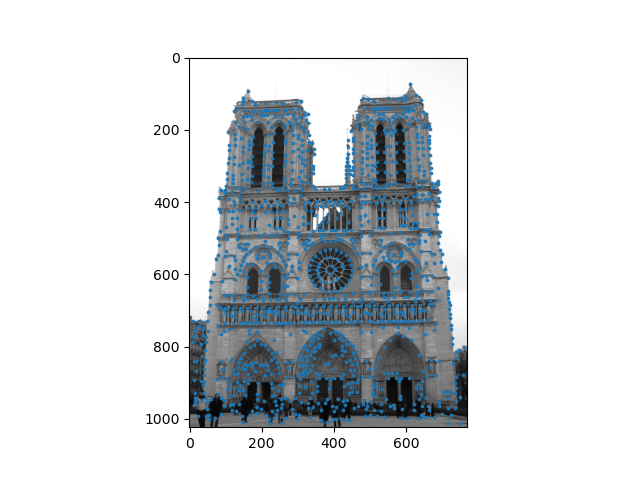
\includegraphics[width=\textwidth]{imgs/notre_dame1.png}
        \caption{Notre Dame 1}
    \end{minipage}
    \begin{minipage}[b]{0.3\textwidth}
        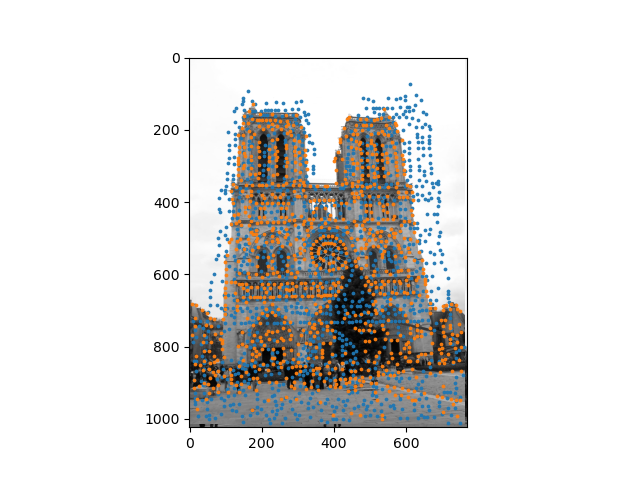
\includegraphics[width=\textwidth]{imgs/notre_dame2.png}
        \caption{Notre Dame 2}
    \end{minipage}
    \begin{minipage}[b]{0.3\textwidth}
        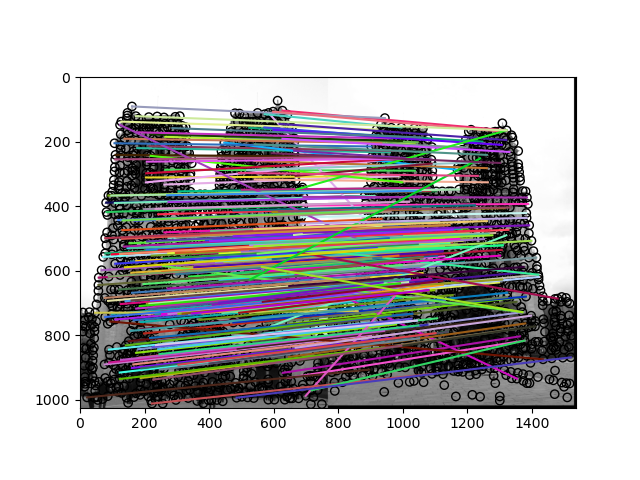
\includegraphics[width=\textwidth]{imgs/notre_dame3.png}
        \caption{Notre Dame match}
    \end{minipage}
    
    \begin{minipage}[b]{0.3\textwidth}
        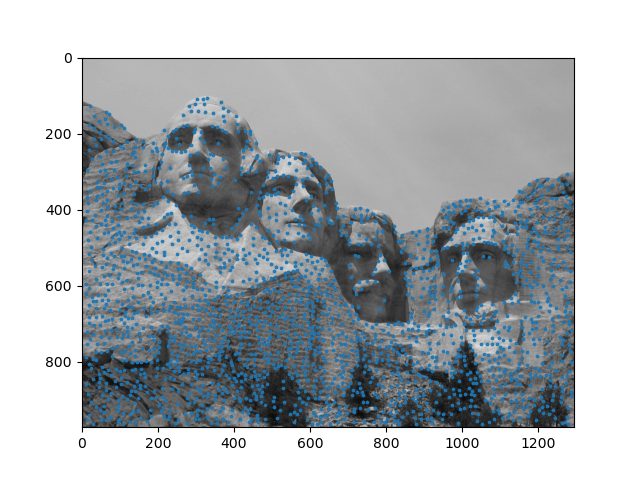
\includegraphics[width=\textwidth]{imgs/mt_rushmore1.png}
        \caption{Mount Rushmore 1}
    \end{minipage}
    \begin{minipage}[b]{0.3\textwidth}
        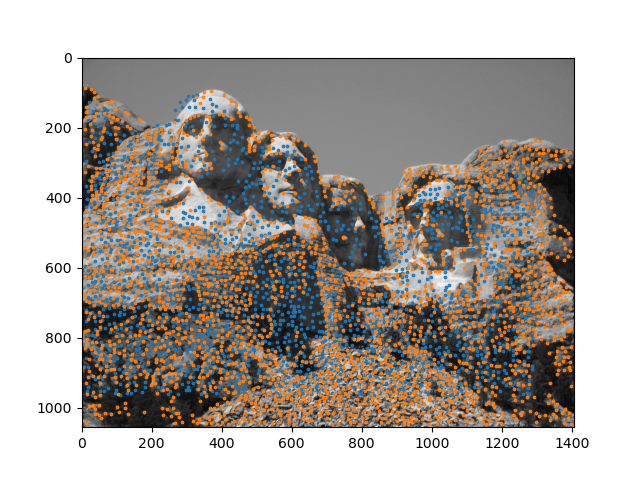
\includegraphics[width=\textwidth]{imgs/mt_rushmore2.png}
        \caption{Mount Rushmore 2}
    \end{minipage}
    \begin{minipage}[b]{0.3\textwidth}
        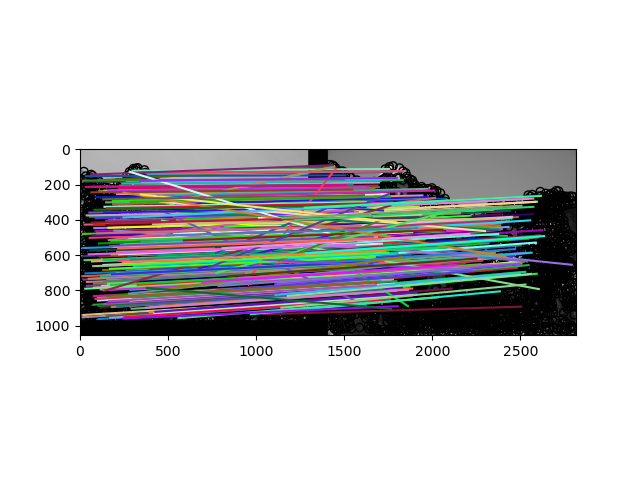
\includegraphics[width=\textwidth]{imgs/mt_rushmore3.png}
        \caption{Mount Rushmore match}
    \end{minipage}
    
    \begin{minipage}[b]{0.3\textwidth}
        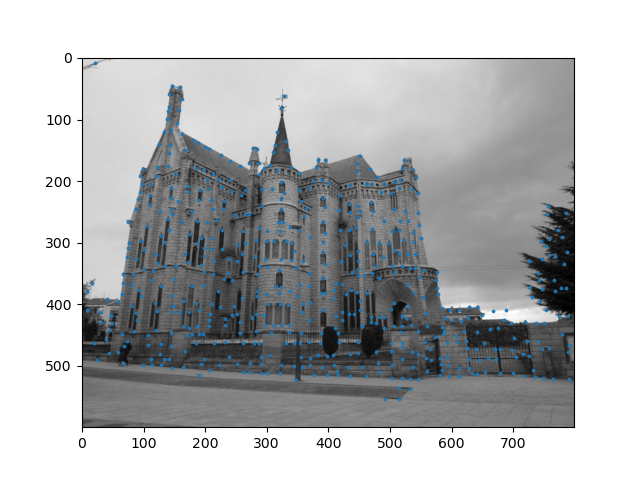
\includegraphics[width=\textwidth]{imgs/e_gaudi1.png}
        \caption{Episcopal Gaudi 1}
    \end{minipage}
    \begin{minipage}[b]{0.3\textwidth}
        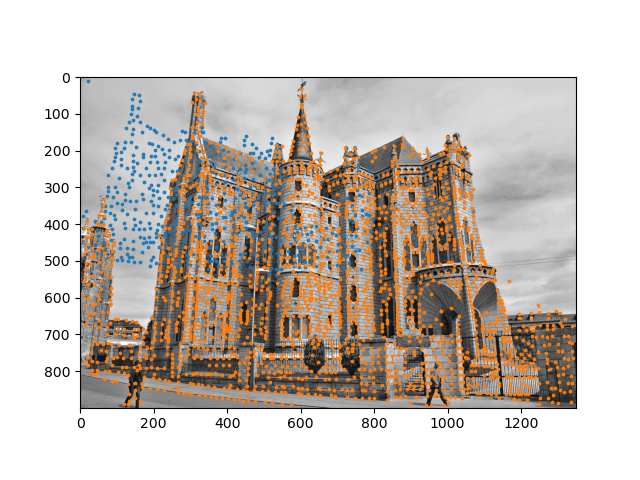
\includegraphics[width=\textwidth]{imgs/e_gaudi2.png}
        \caption{Episcopal Gaudi 2}
    \end{minipage}
    \begin{minipage}[b]{0.3\textwidth}
        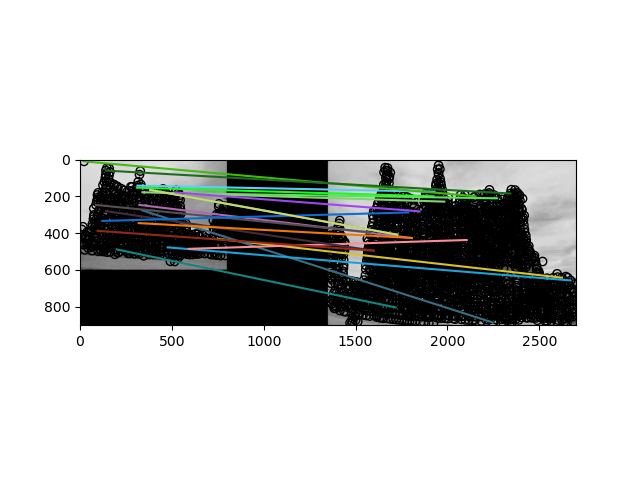
\includegraphics[width=\textwidth]{imgs/e_gaudi3.png}
        \caption{Episcopal Gaudi match}
    \end{minipage}
    \caption{特征匹配可视化结果}
    \label{图1:}
\end{figure}

\subsection{定量结果}
表1总结了在不同图像对上的特征匹配准确率:
\begin{table}[h!]
    \centering
    \caption{特征匹配准确率}
    \label{tab:accuracy}
    \begin{tabular}{ccc}
    \toprule
    \textbf{image} & \textbf{precision} & \textbf{accuracy}\\
    \midrule
    Notre Dame & 0.993&  0.99\\
    Mount Rushmore & 0.944&  0.94\\
    Episcopal Gaudi & 0.151&  0.17\\
    \bottomrule
    \end{tabular}
\end{table}

\section{实验结论:}
准确率的计算是基于提供的 ground truth 匹配进行的。
从结果可以看出,SIFT特征在不同场景下都能取得不错的匹配效果。

我们可以看到,算法在Notre Dame和Mount Rushmore性能表现优异,
但是在图像Episcopal Gaudi表现不尽人意,
而且在该参数下运行速度较慢。
这可能和Harris角点检测算法的局限性有关,因为在该图像两个建筑的距离比较大, 
仰角变动也比较大,可能导致许多特征点匹配失败。

    
    

\section{总结及心得体会:}
通过本次实验,我对局部特征提取与匹配的关键技术有了更深入的理解和体会。

实验过程中,我不仅回顾了 Harris 角点检测和 SIFT 特征描述的理论知识,
更通过实际编程或调用库函数,亲手实现了特征提取和匹配的过程。
这使得我对算法的内部工作原理有了更直观的认识,加深了理论知识的理解。

在 Harris 角点检测部分,我体会到了不同参数
对检测结果的影响。
理解这些参数的作用以及如何进行调优,
对于在实际应用中获得更好的特征点检测效果至关重要。

实验结果表明,SIFT 特征在不同图像对上表现良好,
但也存在一些挑战,例如在光照、视角变化较大的情况下,
匹配准确率可能会受到影响。

\section{对本实验过程及方法、手段的改进建议及展望:}

本次实验成功实现了基于 SIFT 特征的图像匹配,
但也存在一些可以改进和进一步探索的方向。

除了 SIFT,还有许多其他的局部特征检测与描述算法,
如 SURF、ORB、AKAZE 等。
未来的工作可以尝试使用这些算法进行特征匹配,
并与 SIFT 的结果进行比较,分析它们在不同场景下的性能差异。

本实验使用了基本的最近邻匹配方法。
可以考虑引入更鲁棒的匹配策略,
例如结合 RANSAC 等方法剔除误匹配点,进一步提高匹配的准确率。

实验中未对图像进行特殊的预处理。
可以研究不同图像预处理技术
(如噪声滤波、对比度增强等)对特征检测和匹配效果的影响。

\vspace{4cm}
\begin{flushright}
\begin{tabular}{lc}
\sihao{\hei{报告评分:}}& \sihao{\song{~~~~~~}}\\
\sihao{\hei{指导教师签字:}}& \sihao{\song{~~~~~~}}\\
\end{tabular}
\end{flushright}

\newpage

\begin{appendix}
\section{代码示例}

核心代码如代码1所示。

\begin{lstlisting}[caption={student.py}, label={lst:code-example}, captionpos=t, language=python]
  import numpy as np
  import matplotlib.pyplot as plt
  from skimage import feature, img_as_int
  from skimage.measure import regionprops
  import cv2
  from skimage.filters import gaussian, sobel_h, sobel_v
  
  
  def get_interest_points(image, feature_width):
      '''
      Returns a set of interest points for the input image
  
      (Please note that we recommend implementing this function last and using cheat_interest_points()
      to test your implementation of get_features() and match_features())
  
      Implement the Harris corner detector (See Szeliski 4.1.1) to start with.
      You do not need to worry about scale invariance or keypoint orientation estimation
      for your Harris corner detector.
      You can create additional interest point detector functions (e.g. MSER)
      for extra credit.
  
      If you're finding spurious (false/fake) interest point detections near the boundaries,
      it is safe to simply suppress the gradients / corners near the edges of
      the image.
  
      Useful functions: A working solution does not require the use of all of these
      functions, but depending on your implementation, you may find some useful. Please
      reference the documentation for each function/library and feel free to come to hours
      or post on Piazza with any questions
  
          - skimage.feature.peak_local_max
          - skimage.measure.regionprops
  
  
      :params:
      :image: a grayscale or color image (your choice depending on your implementation)
      :feature_width:
  
      :returns:
      :xs: an np array of the x coordinates of the interest points in the image
      :ys: an np array of the y coordinates of the interest points in the image
  
      :optional returns (may be useful for extra credit portions):
      :confidences: an np array indicating the confidence (strength) of each interest point
      :scale: an np array indicating the scale of each interest point
      :orientation: an np array indicating the orientation of each interest point
  
      '''
  
      # TODO: Your implementation here!
      if image.ndim == 3:
          image = cv2.cvtColor(image, cv2.COLOR_BGR2GRAY)
  
      image = img_as_int(image)
  
      Ix = sobel_v(image)
      Iy = sobel_h(image)
      Ix2 = Ix * Ix
      Iy2 = Iy * Iy
      Ixy = Ix * Iy
      
      k = 0.00001 
      sigma = feature_width / 6.0 
      min_distance = int(feature_width / 3) 
      threshold_rate = 0.0005 
      
  
      Sxx = gaussian(Ix2, sigma=sigma)
      Syy = gaussian(Iy2, sigma=sigma)
      Sxy = gaussian(Ixy, sigma=sigma)
  
      det_M = Sxx * Syy - Sxy * Sxy
      trace_M = Sxx + Syy
      harris_response = det_M - k * (trace_M ** 2)
      threshold = threshold_rate * harris_response.max()
      
      coords = feature.peak_local_max(harris_response, min_distance=min_distance, threshold_abs=threshold)
      ys, xs = coords[:, 0], coords[:, 1] # peak_local_max (row, col), (y, x)
  
      border_margin = int(feature_width / 2)
      height, width = image.shape
      valid_indices = np.where(
          (xs >= border_margin) & (xs < width - border_margin) &
          (ys >= border_margin) & (ys < height - border_margin)
      )
      xs = xs[valid_indices]
      ys = ys[valid_indices]
  
      # xs = np.asarray([0])
      # ys = np.asarray([0])
      return xs, ys
  
  
  def get_features(image, x, y, feature_width):
      '''
      Returns a set of feature descriptors for a given set of interest points.
  
      (Please note that we reccomend implementing this function after you have implemented
      match_features)
  
      To start with, you might want to simply use normalized patches as your
      local feature. This is very simple to code and works OK. However, to get
      full credit you will need to implement the more effective SIFT-like descriptor
      (See Szeliski 4.1.2 or the original publications at
      http://www.cs.ubc.ca/~lowe/keypoints/)
  
      Your implementation does not need to exactly match the SIFT reference.
      Here are the key properties your (baseline) descriptor should have:
      (1) a 4x4 grid of cells, each descriptor_window_image_width/4.
      (2) each cell should have a histogram of the local distribution of
          gradients in 8 orientations. Appending these histograms together will
          give you 4x4 x 8 = 128 dimensions.
      (3) Each feature should be normalized to unit length
  
      You do not need to perform the interpolation in which each gradient
      measurement contributes to multiple orientation bins in multiple cells
      As described in Szeliski, a single gradient measurement creates a
      weighted contribution to the 4 nearest cells and the 2 nearest
      orientation bins within each cell, for 8 total contributions. This type
      of interpolation probably will help, though.
  
      You do not need to do the normalize -> threshold -> normalize again
      operation as detailed in Szeliski and the SIFT paper. It can help, though.
  
      Another simple trick which can help is to raise each element of the final
      feature vector to some power that is less than one.
  
      Useful functions: A working solution does not require the use of all of these
      functions, but depending on your implementation, you may find some useful. Please
      reference the documentation for each function/library and feel free to come to hours
      or post on Piazza with any questions
  
          - skimage.filters (library)
  
  
      :params:
      :image: a grayscale or color image (your choice depending on your implementation)
      :x: np array of x coordinates of interest points
      :y: np array of y coordinates of interest points
      :feature_width: in pixels, is the local feature width. You can assume
                      that feature_width will be a multiple of 4 (i.e. every cell of your
                      local SIFT-like feature will have an integer width and height).
      If you want to detect and describe features at multiple scales or
      particular orientations you can add input arguments.
  
      :returns:
      :features: np array of computed features. It should be of size
              [len(x) * feature dimensionality] (for standard SIFT feature
              dimensionality is 128)
  
      '''
  
      # TODO: Your implementation here!
  
      # This is a placeholder - replace this with your features!
      # features = np.asarray([0])
  
      num_interest_points = len(x)
      features = np.zeros((num_interest_points, 128)) # 128 dimensions for SIFT-like descriptor
  
      # Convert image to grayscale if it's color (although input is expected to be grayscale based on notebook)
      if image.ndim == 3:
          image = cv2.cvtColor(image, cv2.COLOR_BGR2GRAY)
  
      # Convert image to float for gradient calculations
      image = img_as_int(image)
  
      # Calculate gradients
      # Using Sobel filters again for consistency with get_interest_points
      Ix = sobel_v(image)
      Iy = sobel_h(image)
  
      # Calculate gradient magnitude and orientation
      magnitude = np.sqrt(Ix**2 + Iy**2)
      # Add a small epsilon to avoid division by zero in arctan2 if both Ix and Iy are 0
      orientation = np.arctan2(Iy, Ix + 1e-6) * 180 / np.pi # Convert to degrees
      # Normalize orientation to be within [0, 360)
      orientation = (orientation + 360) % 360
  
      # Define cell and bin parameters
      num_cells = 4
      num_bins = 8
      cell_width = feature_width // num_cells
      bin_size = 360 // num_bins # Size of each orientation bin in degrees
  
      # Process each interest point
      for i in range(num_interest_points):
          # Get the coordinates of the current interest point
          px, py = x[i], y[i]
  
          # Define the bounding box for the feature window
          # Need to be careful with boundary conditions
          half_width = feature_width // 2
          min_x = max(0, px - half_width)
          max_x = min(image.shape[1] - 1, px + half_width -1) # -1 because max_x is inclusive index
          min_y = max(0, py - half_width)
          max_y = min(image.shape[0] - 1, py + half_width -1) # -1 because max_y is inclusive index
  
          # Ensure window size is correct even at boundaries
          # This might require padding the image or adjusting the window size/handling points near border
          # For simplicity here, we'll just take the available window and handle potential smaller size
          # A more robust implementation might pad the image.
  
          # Extract the local patch
          # Note: Slicing includes start but excludes end. Adjust max indices accordingly.
          patch_mag = magnitude[min_y : max_y + 1, min_x : max_x + 1]
          patch_ori = orientation[min_y : max_y + 1, min_x : max_x + 1]
  
          # Ensure patch is exactly feature_width x feature_width. If not, there's likely an issue with
          # how interest points near the border were handled or how min/max were calculated.
          # Given the border suppression in get_interest_points, this window *should* be full size
          # if border_margin >= feature_width / 2.
          # For now, proceed assuming full size or handle potential smaller size in histogramming.
  
          descriptor = np.zeros(num_cells * num_cells * num_bins) # 4x4 grid * 8 bins = 128
  
          # Build histograms for each cell
          # Instead of iterating through cells then pixels, iterate through pixels and contribute to cells/bins
          # We need patch-relative coordinates for interpolation
          patch_height, patch_width = patch_mag.shape
  
          # Define Gaussian weighting window
          # Sigma for Gaussian is typically half the window size
          sigma_spatial = feature_width / 2.0
          y_coords, x_coords = np.indices(patch_mag.shape)
          # Calculate distance from the center of the patch (which aligns with the interest point)
          # Center of patch is at (half_width - 0.5, half_width - 0.5) if patch is feature_width x feature_width
          patch_center_r = patch_height / 2.0 - 0.5
          patch_center_c = patch_width / 2.0 - 0.5
          distances_sq = (x_coords - patch_center_c)**2 + (y_coords - patch_center_r)**2
          gaussian_weights_patch = np.exp(-distances_sq / (2 * sigma_spatial**2))
  
          # Process each pixel in the patch
          # Coordinates relative to the top-left of the patch (0 to feature_width-1)
          for r in range(patch_height):
              for c in range(patch_width):
                  mag = patch_mag[r, c]
                  ori = patch_ori[r, c]
                  gaussian_weight = gaussian_weights_patch[r, c]
  
                  # Apply Gaussian weight to the magnitude
                  weighted_mag = mag * gaussian_weight
  
                  # Normalize orientation to be within [0, 360) for bin calculation
                  ori = (ori + 360) % 360
  
                  # Calculate the float bin index (0 to num_bins - epsilon)
                  float_bin_index = ori / bin_size
  
                  # Get the two nearest integer bin indices
                  bin1_index = int(np.floor(float_bin_index)) % num_bins
                  bin2_index = int(np.ceil(float_bin_index)) % num_bins
  
                  # Calculate orientation weights for the two bins
                  # Fractional part of the float bin index gives the position between the two bins
                  fractional_part_ori = float_bin_index - np.floor(float_bin_index)
                  ori_weight1 = (1 - fractional_part_ori) # Weight for bin1_index
                  ori_weight2 = fractional_part_ori     # Weight for bin2_index
  
                  # Calculate spatial position relative to the top-left of the feature window (0 to feature_width-1)
                  # and then map to cell coordinates (0 to num_cells)
                  # Pixel (r, c) in patch is at (c, r) relative to patch top-left
                  # Map patch coordinates to cell coordinates. Cell centers are at (0.5, 1.5, 2.5, 3.5) * cell_width + cell_width/2
                  # Pixel (c, r) in patch falls into a cell with top-left at floor(c/cell_width)*cell_width, floor(r/cell_width)*cell_width
  
                  # Calculate float cell coordinates based on pixel position within the feature window (0 to num_cells)
                  # Pixel (c, r) is at spatial location (c+0.5, r+0.5) within the patch (0 to feature_width)
                  float_cell_x = (c + 0.5) / cell_width
                  float_cell_y = (r + 0.5) / cell_width
  
                  # Get the two nearest integer cell indices in each dimension (0 to num_cells)
                  cell1_x = int(np.floor(float_cell_x))
                  cell2_x = int(np.ceil(float_cell_x))
                  cell1_y = int(np.floor(float_cell_y))
                  cell2_y = int(np.ceil(float_cell_y))
  
                  # Calculate spatial weights for the four cells (bilinear interpolation)
                  fractional_part_x = float_cell_x - np.floor(float_cell_x)
                  fractional_part_y = float_cell_y - np.floor(float_cell_y)
  
                  # Weights for the 4 target cells based on bilinear interpolation
                  spatial_weight11 = (1 - fractional_part_x) * (1 - fractional_part_y) # cell1_x, cell1_y
                  spatial_weight21 = fractional_part_x * (1 - fractional_part_y)     # cell2_x, cell1_y
                  spatial_weight12 = (1 - fractional_part_x) * fractional_part_y     # cell1_x, cell2_y
                  spatial_weight22 = fractional_part_x * fractional_part_y         # cell2_x, cell2_y
  
                  # Add weighted magnitude to the corresponding bins in the descriptor
                  # Iterate over the 4 target cells and 2 target orientation bins
                  target_contributions = [
                      (cell1_x, cell1_y, spatial_weight11, bin1_index, ori_weight1),
                      (cell1_x, cell1_y, spatial_weight11, bin2_index, ori_weight2),
                      (cell2_x, cell1_y, spatial_weight21, bin1_index, ori_weight1),
                      (cell2_x, cell1_y, spatial_weight21, bin2_index, ori_weight2),
                      (cell1_x, cell2_y, spatial_weight12, bin1_index, ori_weight1),
                      (cell1_x, cell2_y, spatial_weight12, bin2_index, ori_weight2),
                      (cell2_x, cell2_y, spatial_weight22, bin1_index, ori_weight1),
                      (cell2_x, cell2_y, spatial_weight22, bin2_index, ori_weight2),
                  ]
  
                  for cur_cx, cur_cy, spatial_w, bin_idx, ori_w in target_contributions:
                      # Ensure cell indices are within the 0-3 range
                      if 0 <= cur_cx < num_cells and 0 <= cur_cy < num_cells:
                           # Calculate the final weighted magnitude contribution
                           final_weighted_mag = weighted_mag * spatial_w * ori_w
  
                           # Calculate the index in the flattened descriptor
                           descriptor_index = (cur_cy * num_cells + cur_cx) * num_bins + bin_idx
  
                           # Add to the descriptor
                           descriptor[descriptor_index] += final_weighted_mag
  
  
          # Normalize the descriptor to unit length
          # Add a small epsilon to the norm to prevent division by zero for uniform patches
          norm = np.linalg.norm(descriptor) + 1e-6
          descriptor /= norm
  
          # Apply thresholding and re-normalization (SIFT specific)
          threshold_value = 0.2
          descriptor[descriptor > threshold_value] = threshold_value
  
          # Second normalization after thresholding
          norm = np.linalg.norm(descriptor) + 1e-6
          descriptor /= norm
  
          # Assign the computed descriptor to the features array
          features[i, :] = descriptor
  
  
      return features
  
  
  def match_features(im1_features, im2_features):
      '''
      Implements the Nearest Neighbor Distance Ratio Test to assign matches between interest points
      in two images.
  
      Please implement the "Nearest Neighbor Distance Ratio (NNDR) Test" ,
      Equation 4.18 in Section 4.1.3 of Szeliski.
  
      For extra credit you can implement spatial verification of matches.
  
      Please assign a confidence, else the evaluation function will not work. Remember that
      the NNDR test will return a number close to 1 for feature points with similar distances.
      Think about how confidence relates to NNDR.
  
      This function does not need to be symmetric (e.g., it can produce
      different numbers of matches depending on the order of the arguments).
  
      A match is between a feature in im1_features and a feature in im2_features. We can
      represent this match as a the index of the feature in im1_features and the index
      of the feature in im2_features
  
      Useful functions: A working solution does not require the use of all of these
      functions, but depending on your implementation, you may find some useful. Please
      reference the documentation for each function/library and feel free to come to hours
      or post on Piazza with any questions
  
          - zip (python built in function)
  
      :params:
      :im1_features: an np array of features returned from get_features() for interest points in image1
      :im2_features: an np array of features returned from get_features() for interest points in image2
  
      :returns:
      :matches: an np array of dimension k x 2 where k is the number of matches. The first
              column is an index into im1_features and the second column is an index into im2_features
      :confidences: an np array with a real valued confidence for each match
      '''
  
      # TODO: Your implementation here!
  
      # These are placeholders - replace with your matches and confidences!
  
      matches = []
      confidences = []
  
      # Iterate through each feature in the first image
      for i, feature1 in enumerate(im1_features):
          # Calculate distances to all features in the second image
          distances = np.linalg.norm(im2_features - feature1, axis=1)
  
          # Find the indices of the two smallest distances
          # Use argpartition to find the indices of the k smallest elements efficiently
          if len(distances) < 2:
               # Need at least two features in im2 to calculate ratio
               continue
  
          # Get indices of the two smallest distances
          nearest_indices = np.argpartition(distances, 1)[:2]
  
          # Ensure we get the two actual smallest distances in correct order
          if distances[nearest_indices[0]] > distances[nearest_indices[1]]:
              nearest_indices = nearest_indices[[1, 0]] # Swap if necessary
  
          d1 = distances[nearest_indices[0]] # Distance to nearest neighbor
          d2 = distances[nearest_indices[1]] # Distance to second nearest neighbor
  
          # Apply Nearest Neighbor Distance Ratio (NNDR) test
          # A small ratio indicates a good match
          if d2 > 0: # Avoid division by zero
              ratio = d1 / d2
          else:
              # If second nearest neighbor has 0 distance, it's likely an identical feature
              # Treat this as a very confident match (ratio approaches 0)
              ratio = 0
  
          # Set a threshold for the ratio. This value may need tuning.
          # A common starting point is 0.8
          nndr_threshold = 0.8
  
          if ratio < nndr_threshold:
              # This is considered a valid match
              matches.append([i, nearest_indices[0]])
  
              # Calculate confidence (e.g., 1 - ratio, or based on ratio inverse)
              # Lower ratio means higher confidence
              confidence = 1.0 - ratio # Example confidence calculation
              confidences.append(confidence)
  
      # Convert lists to numpy arrays
      matches = np.asarray(matches)
      confidences = np.asarray(confidences)
  
      # Optional: Sort matches by confidence in descending order
      # (Useful for evaluation which might only look at top N matches)
      # sort_indices = np.argsort(confidences)[::-1]
      # matches = matches[sort_indices]
      # confidences = confidences[sort_indices]
  
      return matches, confidences
\end{lstlisting}

\end{appendix}

\end{document}
